\chapter{Eksperimental Opsætning}
Denne sektion har til formål at beskrive opgavens eksperimentale opsætning dertil hvilke billeder der er anvendt og hvordan metoderne er afprøvet.
\section{Anvendte Billeder}
De udvalgte billeder, som opgavens resultater bygger på, er taget fra overflyvningen af én mark. De udvalgte billeder, består af 10 billeder, taget længst væk fra jorden, 4 billeder taget næst-længst fra jorden og 4 billeder taget tættest fra jorden. I billede sættet består hver højdeforskel af mindst ét sæt billeder, hvor der er markante strukturer i billedet, fx. en partielt høstet del af marken, og mindst ét sæt billeder hvor hele billedet er dækket af korn.
\begin{figure}[H]
    \centering
    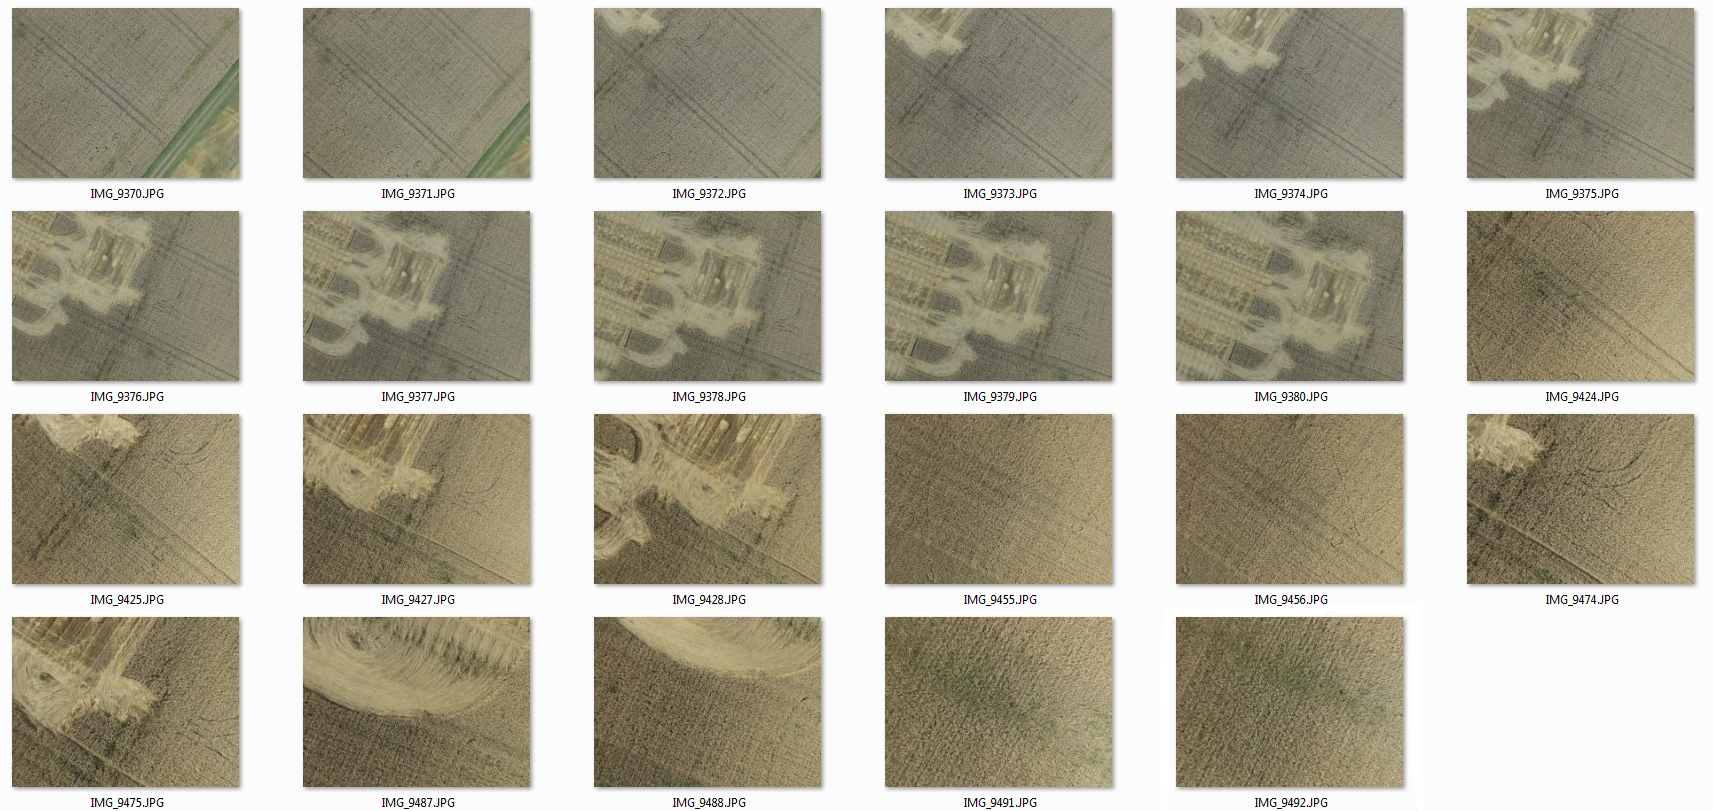
\includegraphics[width=1\textwidth]{fig/43a.png}
    \vspace{-0.5em}   
    \begin{center}
    \caption{\textcolor{gray}{\footnotesize \textit{Udvalgt billedesæt}}}
    \label{fig:lindblob}
     \end{center}
  \end{figure}
       \vspace{-2.7em}
\noindent
\section{Metode Opsætning}
Følgende er kombinationer af metoderne afprøvet på ovenstående billedsæt:
\begin{itemize}
\item{Moravec $\rightarrow$ SIFT}
\item{Harris $\rightarrow$ SIFT}
\item{Difference of Gaussian $\rightarrow$ SIFT}
\item{Determinant of Hessian $\rightarrow$ SURF}
\end{itemize}
<FEJLKILDER>
<test kombination af billederne> \\
<hvad er testet, rotation, struktur, skala>